\documentclass[a4paper,12pt]{article}

\usepackage{titlesec}
\titleformat{\paragraph}[runin]
{\normalfont\bfseries}{\thesubsection.\arabic{paragraph}}{1em}{}

\setcounter{paragraph}{0}

\usepackage{hyperref}
\usepackage[utf8]{inputenc}
\usepackage[T1]{fontenc}
\usepackage[french]{babel}
\usepackage{graphicx}
\usepackage{titling}

\usepackage{geometry}
\geometry{top=2cm, bottom=2cm, left=2.5cm, right=2.5cm}

\begin{document}
	\begin{titlepage}
		\centering
		{\Huge \textbf{Jeu Projet 2}} \\[1.5cm]
		Olivier Cochard \\
		\today \\[2cm]
		
		
		
		
		{\Large Rapport de projet} \\[0.5cm]
		{\large \textit{Université de Caen Normandie}} \\[2cm]
		\includegraphics[width=0.3\textwidth]{Logo_Université_de_Caen_Normandie_2018}
		
		
		
		\vfill
		{\small Ce rapport a été rédigé dans le cadre du projet de Projet 2, encadré par ADDAD Youva.}
	\end{titlepage}
	
	
	
\newpage

\tableofcontents
	
\newpage

\section{Introduction}
Ce rapport présente la conception et a réalisation d'un jeu de Tron multi-joueurs dans le cadre d'un projet d'Intelligence Artificielle. Ce travail a été réalisé en monôme et vise à étudier l’impact des coalitions entre joueurs dans un environnement compétitif. L'objectif principal est de développer une application robuste, modulaire et extensible, permettant d’évaluer la performance des stratégies d’équipes en fonction de différents paramètres, tels que la profondeur de recherche, la taille des équipes et les dimensions de la grille.

Le jeu de Tron est une variante multi-joueurs du célèbre jeu de serpent, où chaque joueur ou IA contrôle un pion laissant derrière lui un obstacle à chaque déplacement. Ce projet se concentre sur l’implémentation de différents algorithmes d'IA avancés qui sont les suivant: MaxN et Paranoid. Ainsi que l’implémentation de leur extension pou gérer des parties comprenant des équipes. L’enjeu scientifique consiste à analyser l’influence de la profondeur de raisonnement sur les performances des joueurs, en fonction de la taille des coalitions et de la grille de jeu.

L'architecture que j'ai choisi repose sur une séparation claire entre modèle, vue et contrôleur ainsi qu'un modèle Observeur et Observable. Cette architecture garanti une indépendance entre les composants et facilite les extensions futures.
Ce rapport détaille les choix de conceptions, algorithmes clés et améliorations possibles pour enrichir le projet.

\section{Spécifications et Conception}
\subsection{Diagramme de classe}
Le principe de l'Observeur et l'Observable ici, permet de gérer la communication entre Plateau et toutes les entités de ma grille. Après avoir reçut les information, mon Observeur se met à jour en conséquence et agis ensuite sur les Observables concernés.

	\begin{figure}[h!]
		\centering	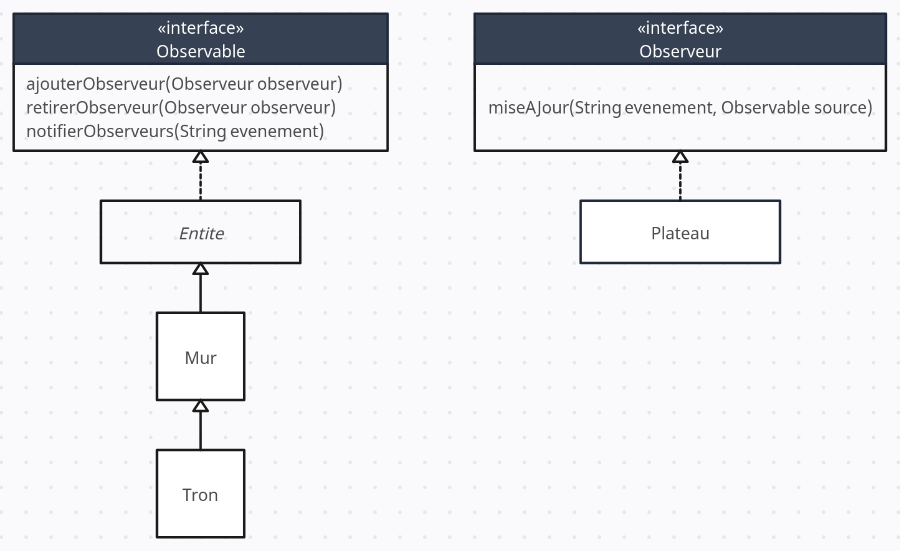
\includegraphics[width=0.5\linewidth]{DiagObserveurObservable}
		\caption{Diagramme de classe Observeur et Observable}
	\end{figure}
	
Les classes MaxN, MaxNSOS, Paranoide et ParanoideSOS ont toute l'implémentation de l'interface IA.java. Voici le diagramme de classe illustrant mes propos.
	
	\begin{figure}[h!]
		\centering	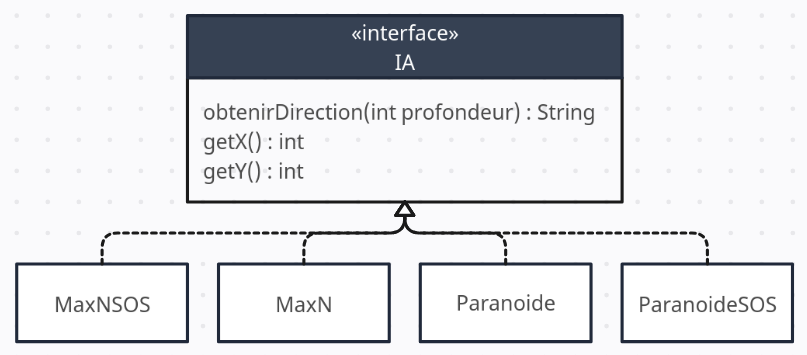
\includegraphics[width=0.5\linewidth]{DiagIA}
		\caption{Diagramme de classe des IA}
	\end{figure}
	
L'interface TronPlacementStrategie est implémentée par les classes TronPlacementChaos, TronPlacemebtEquilibre et TronPlacementOptimale.

\begin{figure}[h!]
		\centering	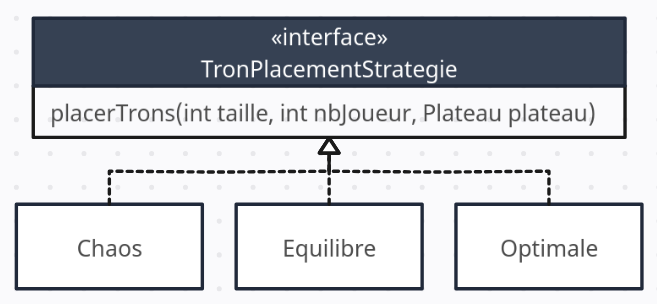
\includegraphics[width=0.5\linewidth]{DiagPlacement}
		\caption{Diagramme de classe du stratégie pattern de qui gère l'apparition des trons sur la grille en début de partie}
	\end{figure}

\subsection{Diagramme de cas}
Un tour classique se passe de la façon suivante:
le tron courant doit renvoyer un String direction, si c'est un joueur il devra rentrer une direction en chaine de caractère dans le terminal et si c'est un bot alors la fonction obtenirDirection(int profondeur) en retournera une.

	\begin{figure}[h!]
		\centering	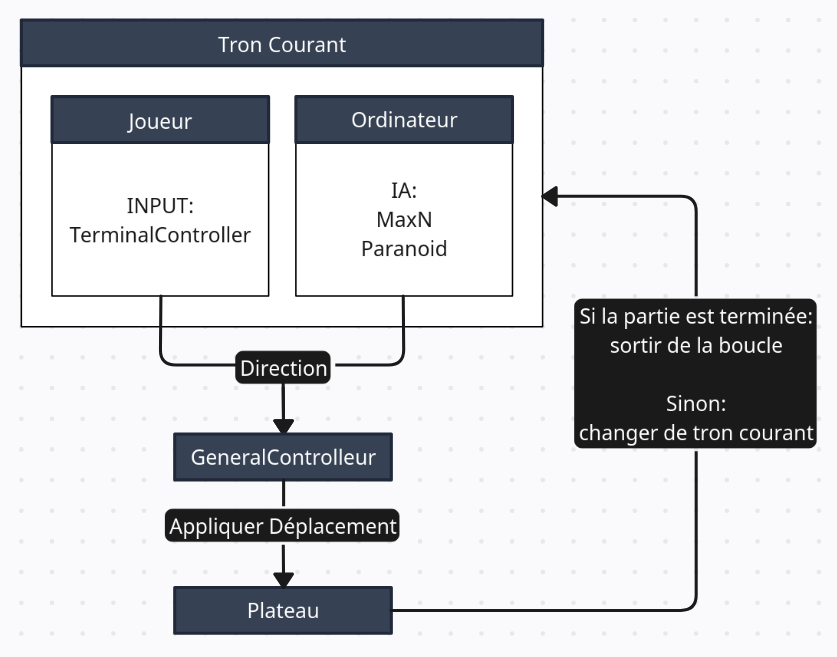
\includegraphics[width=0.5\linewidth]{DiagTourClassique}
		\caption{Diagramme de cas d'un tour de jeu classique}
	\end{figure}


\subsection{Interface graphique}
Mon interface graphique est très simpliste, je n'ai pas voulu concentrer mes efforts dessus. 
J'utilise un JFrame qui gère la fenêtre et un GamePanel enfant de la classe JPanel qui me permet de faire le rendu graphique de la grille et ses entités.
Une cellule verte avec un chiffre représente un joueur vivant, une cellule rouge avec une croix représente un joueur mort. Un mur est représenté par la couleur blanche et pour finir une cellule noire représente une case libre.
Cette interface graphique respecte bien les principes SOLID et MVC.

\begin{figure}[h!]
		\centering	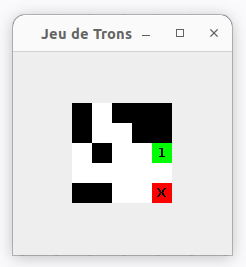
\includegraphics[width=0.3\linewidth]{InterfaceGraphique}
		\caption{Diagramme de cas d'un tour de jeu classique}
	\end{figure}

\section{Intelligences artificielles et stratégie}
\subsection{Intelligences artificielles}
\subsubsection{MaxN}
L'algorithme MaxN est une extension de l'algorithme Minimax adaptée pour les jeux à plus de 2 joueurs. Contrairement à Minimax qui suppose une opposition binaire, MaxN permet à chaque joueurs de maximiser sa propre fonction d'évaluation indépendamment des autres.
MaxN est adapté aux jeux multi-joueurs sans alliances, mais sa complexité explose avec la profondeur de recherche et le nombre de joueurs.
\subsubsection{Paranoid}
L'algorithme Paranoid est une autre approche pour les jeux à plusieurs, comme son nom l'indique il est paranoïaque et a l'impression que tout le monde est en alliance contre lui. Le joueur maximise son score tandis que les autres joueurs le minimisent. C'est une généralisation de Minimax ou les autres joueurs sont considérés comme un seul adversaire. Cet algorithme est plus efficace que MaxN contre les adversaires hostiles avec son comportement défensif.
\subsubsection{Extension SOS}
L'extension SOS de ces algorithmes permet d'intégrer des mécanismes de coalition pour réduire l'explosion combinatoire. 
SOS avec MaxN permet de partager un objectif commun avec l'équipe, le gros avantage est une réduction partielle de la complexité mais est assez difficile à équilibrer à cause du choix des poids.
Avec Paranoid les alliers de l'IA font monter le score, il y a donc moins de joueurs qui minimisent son score. Le gros avantage est le fait de prendre en compte les alliers tandis qu'il peut être limité en cas d'alliances dynamiques.
\subsection{Stratégie}
J'ai utilisé un pattern stratégie qui me permet de choisir la règle qui défini comment est gérée l'apparition des trons sur la grille en début de partie.
\subsubsection{Chaos}
Cette classe positionne les trons aléatoirement sur une grille en faiant attention à ne pas écraser les trons, c'est à dire définir une position d'apparition à condition que celle-ci soit libre.

\begin{figure}[h!]
		\centering	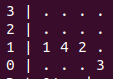
\includegraphics[width=0.2\linewidth]{Chaos}
		\caption{Exemple de placement Chaos sur une grille de taille 4 avec 4 joueurs}
	\end{figure}
		
J'utilise cette stratégie lors de mes analyses afin d'obtenir des situations aléatoires et donc des statistiques pertinentes.
	
\subsubsection{Equilibré}
Cette stratégie est très similaire à Chaos, à la différence prêt qu'une vérification est effectuée, tous les joueurs doivent avoir au moins taille/nbJoueur cellules de distance entre les joueurs.

\begin{figure}[h!]
		\centering	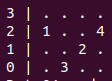
\includegraphics[width=0.2\linewidth]{Equilibre}
		\caption{Exemple de placement Equilibré sur une grille de taille 4 avec 4 joueurs}
	\end{figure}
	
\subsubsection{Optimale}
Cette dernière classe n'a rien à voir avec les précédentes, elle choisi le placement selon des règles fixes. Elle essaie de positionner les trons en symétrie. 

Si le nombre de joueurs est <= 4, il va positionner les joueurs dans les angles.
Si le nombre de trons <= 8 alors celui ci va prioriser les cotés à équidistance (approximatif si grille impaire) des angles.

Et pour finir si le nombre est <= 9 alors en cas de taille de grille impaire, un joueur sera placé au centre (approximatif si grille paire).

\begin{figure}[h!]
		\centering	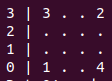
\includegraphics[width=0.2\linewidth]{Optimale_1}
		\caption{Exemple de placement Optimal sur une grille de taille 4 avec 4 joueurs}
	\end{figure}
	
	\begin{figure}[h!]
		\centering	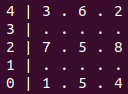
\includegraphics[width=0.2\linewidth]{Optimale_2}
		\caption{Exemple de placement Optimal sur une grille de taille 5 avec 9 joueurs}
	\end{figure}

Sur cette dernière image on observe bien l'ordre de placement.

Son manque d'aléatoire m'a permit d'expérimenter mes IA dans des situations toujours similaires afin d'observer les changement dans leurs comportements.
	
\newpage
\section{Expérimentations et question scientifique}
\subsection{Introduction}
Pour analyser correctement j'ai analysé 3 statistiques intéressantes le taux de victoire, la durée moyenne d'une partie et le temps moyen de calcul pour obtenir la direction renvoyée par les IA. J'ai donc analysé ces statistiques en fonction de 3 paramètres pertinents qui sont les suivants: nombre de joueurs, taille de la grille et profondeur de recherche.
\subsection{Taux de victoire}
\subsubsection{Taille des équipes}
\begin{figure}[h!]
		\centering	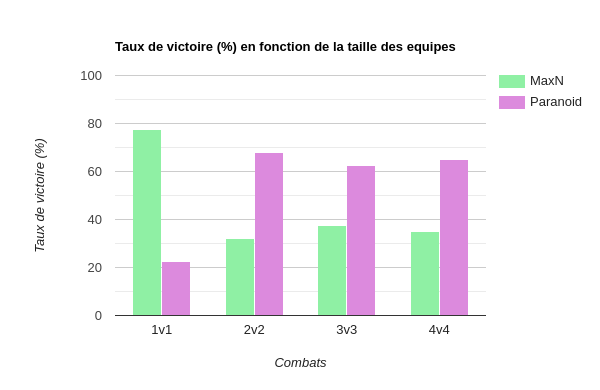
\includegraphics[width=0.5\linewidth]{TauxVictoireEquipe}
		\caption{Graphique étudiant le taux de victoire de MaxN vs Paranoid suivant la taille des équipes, taille de grille 20, profondeur 3, pour 10000 analyses}
	\end{figure}
On observe qu'en 1 contre 1, MaxN prend domine très largement, tandis que le comportement "tous contre un" de Paranoid la rend trop défensive.
En 2v2 Paranoid devient bien meilleure, le fait de traiter tous les autres joueurs comme des ennemis elle est plus aggressive. MaxN perd en efficacité car elle tente d'optimiser pour tous les joueurs, et prend des décisions "trop coopératives".
La tendance ce confirme en 3v3 et 4v4, MaxN à l'inverse de Paranoid perd en agressivité quand les équipes sont plus grandes.
MaxN est plus forte en 1v1 et peine à jouer en équipe par rapport à Paranoid.

\newpage

\subsubsection{Profondeur de recherche}
\begin{figure}[h!]
		\centering
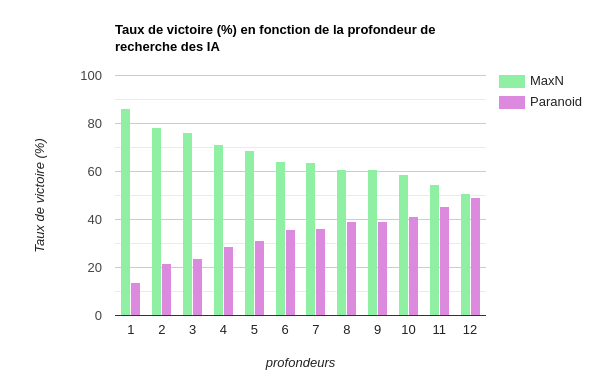
\includegraphics[width=0.5\linewidth]{TauxVictoireProfondeur}
		\caption{Graphique étudiant le taux de victoire de MaxN vs Paranoid suivant la profondeur de recherche, taille de grille 20, 1v1, pour 10000 analyses}
	\end{figure}
On observe que MaxN domine à faible profondeur, mais son avantage diminue avec l'augmentation de la profondeur. Paranoid s’améliore donc progressivement, les deux IA ont un taux de victoire équilibré vers la profondeur 11-12. Vers une stratégie optimale, MaxN reste légèrement meilleur, car elle évite mes erreurs grossières cependant Paranoid compense par son agressivité mieux calculée.
\subsubsection{Taille de la grille}
\begin{figure}[h!]
		\centering
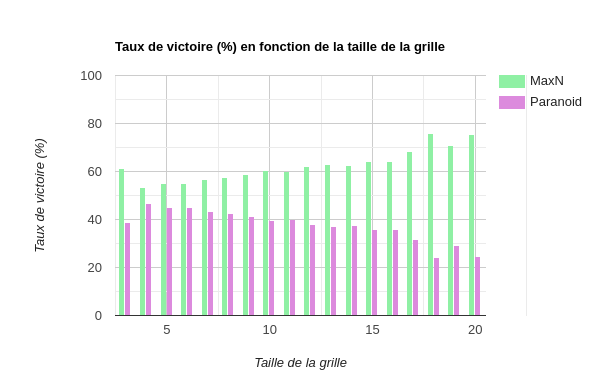
\includegraphics[width=0.5\linewidth]{TauxVictoireTaille}
		\caption{Graphique étudiant le taux de victoire de MaxN vs Paranoid suivant la taille de la grille, profondeur 3, 1v1, pour 10000 analyses}
	\end{figure}
MaxN domine de encore plus sur les grandes cartes, ça lui offre plus de possibilités stratégiques, elle esquive mieux les pièges et contrôle mieux l'espace. Paranoid s'en sort mieux sur les petites cartes en exploitant le manque d'option de fuite, elle se fait piéger plus facilement dans les situations où MaxN peut anticiper plusieurs coups à l'avance. 
\subsubsection{Conclusion du taux de victoire}
MaxN domine plus en 1v1 et a plus de difficultés lors de coalitions. Paranoid est de plus en plus efficace avec une grande profondeur de recherche et le combien devient équilibré vers la profondeur 11-12. Elle est aussi très largement dominée quand la profondeur est petite. La taille de la grille a un impact énorme sur l’issue des combats, Paranoid arrive à rivaliser avec MaxN avec des petites grilles mais plus celle-ci augmente plus MaxN a de l'espace pour piéger son adversaire.

\subsection{Temps de calcul moyen}
\subsubsection{Taille des équipes}
\begin{figure}[h!]
		\centering	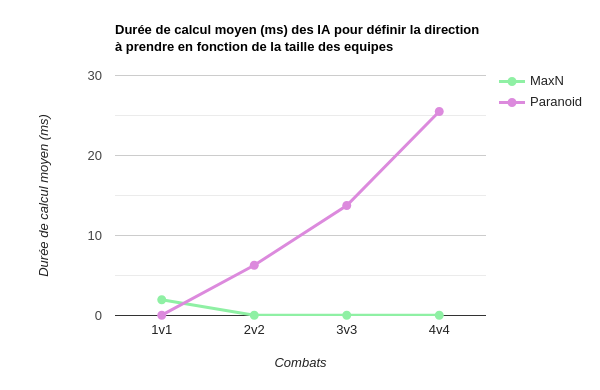
\includegraphics[width=0.5\linewidth]{TempsCoupEquipe}
		\caption{Graphique étudiant le temps de calcul moyen d'un coup lors du 1v1 MaxN vs Paranoid suivant la taille des équipes, taille de grille 20, profondeur 3, pour 10000 analyses}
		\end{figure}
MaxN est ultra-rapide en multijoueur mais lente en 1v1. A l'inverse de Paranoid qui est rapide en 1v1 mais extrêmement lente dès que le nombre de joueurs augmente. Elle est 600x plus lente en 4v4 (25.492 ms) qu'en 1v1 (0.041 ms).
Paranoid considère tous les joueurs comme des adversaires c'est pourquoi sa complexité devient catastrophique en équipe.
MaxN utilise une approximation pour éviter l'explosion combinatoire.
Paranoid domine le 1v1 tandis que MaxN est meilleure pour le multijoueur.

\subsubsection{Profondeur de recherche}
\begin{figure}[h!]
		\centering	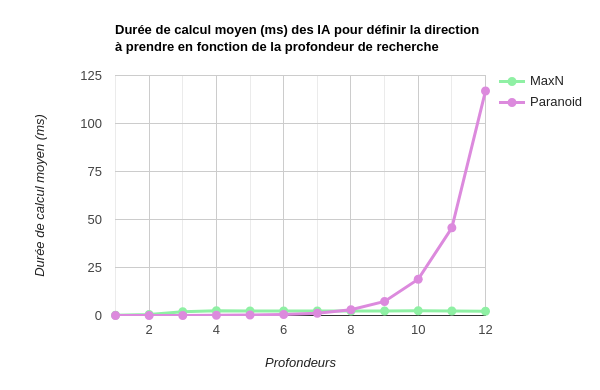
\includegraphics[width=0.5\linewidth]{TempsCoupProfondeur}
		\caption{Graphique étudiant le temps de calcul moyen d'un coup lors du 1v1 MaxN vs Paranoid suivant la profonde de recherche, taille de grille 20, pour 10000 analyses}
		\end{figure}
MaxN est capé à 3 profondeur max pour éviter les temps de calculs, d'après son évolution environ x + 1 = x*4 sa croissance est encore plus rapide que Paranoid, la valeur atteinte par Paranoid en profondeur 12 (116.966 ms) aurait été environ atteinte en profondeur 6 pour MaxN. 

\subsubsection{Taille de la grille}
\begin{figure}[h!]
		\centering	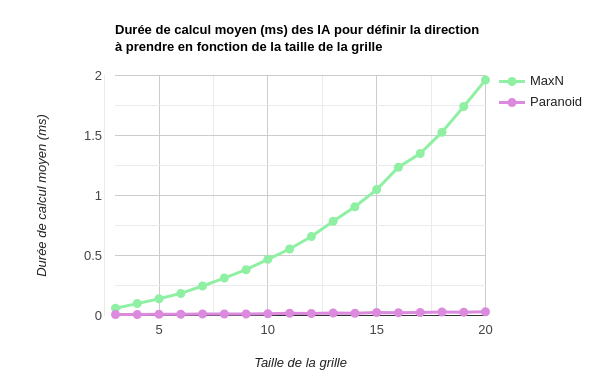
\includegraphics[width=0.5\linewidth]{TempsCoupTaille}
		\caption{Graphique étudiant le temps de calcul moyen d'un coup lors du 1v1 MaxN vs Paranoid suivant la taille de la grille, profondeur 3, pour 10000 analyses}
		\end{figure}
MaxN a une croissance linéaire car il y de plus en plus de cases à étudier. Paranoid e concentre plutôt sur un seul adversaire et donc elle est moins sensible à l'expansion de la grille.

\subsubsection{Conclusion temps de calcul moyen d'un coup}
la taille des équipes a une grosses influence sur le temps de calcul, Paranoid a plus d'adversaires à surveiller tandis que MaxN est optimisé pour éviter l'explosion combinatoire.
La profondeur de recherche a une influence impressionnante sur le temps de calcul, les croissances sont exponentielles (sans prendre en compte le blocage volontaire de MaxN), MaxN a une croissance plus importante que Paranoid.
A propos de la taille de la grille sont influence est très légère voir nulle. Sa croissance est linéaire pour Paranoid et stable pour MaxN.

\subsection{Durée moyenne d'une partie}
Pour la suite des expérimentations je teste des affrontements d'IA contre elles-mêmes afin de mesurer leurs agressivités.
\subsubsection{Taille des équipes}
\begin{figure}[h!]
		\centering	\includegraphics[width=0.5\linewidth]{DuréePartieEquipe}
		\caption{Graphique étudiant lors d'un 1v1 d'une IA contre elle-même suivant la taille des équipes, taille de grille 20, profondeur 3, pour 10000 analyses}
		\end{figure}
En 1v1 MaxN est plus prudente et fait plus durer la partie. Paranoid devient compétitive en multijoueur grâce à son agressivité.

\newpage

\subsubsection{Profondeur de recherche}
\begin{figure}[h!]
		\centering	\includegraphics[width=0.5\linewidth]{DuréePartieProfondeur}
		\caption{Graphique étudiant lors d'un 1v1 d'une IA contre elle-même suivant la profondeur de recherche, taille de grille 20, pour 10000 analyses}
		\end{figure}
Le blocage de profondeur maximale de MaxN fausse les résultats, normalement la durée de survie devrait croitre. Paranoid dépend fortement de la profondeur, elle apprend à survivre plus longtemps en voyant plus loin.

\subsubsection{Taille de la grille}
\begin{figure}[h!]
		\centering	\includegraphics[width=0.5\linewidth]{DuréePartieTaille}
		\caption{Graphique étudiant lors d'un 1v1 d'une IA contre elle-même suivant la taille de la grille, profondeur de recherche 3, pour 10000 analyses}
		\end{figure}
Pour les petites grilles (3x3 à 8x8) Paranoid est meilleur en survie que MaxN. Quand les espaces sont moins restreints MaxN excelle. Elle est meilleure en gestion de l'espace et moins vulnérable aux pièges à long terme. A coté Paranoid se disperse plus.

\newpage

\subsubsection{Conclusion durée moyenne d'une partie}
Pour conclure, la taille de la grille est un facteur déterminant, dans les petites grilles Paranoid surclasse MaxN et MaxN reprend l'avantage dans les grandes grilles.
Les résultats de Paranoid en fonction de l'impact de la profondeur prouve son intelligence tactique croissante, à coté la limitation volontaire de MaxN la prive de son potentiel.
D'après le graphique suivant le mode de jeu, MaxN est plus prudente en 1v1 tandis que Paranoid rattrape MaxN en multijoueur grâce à son agressivité.

\subsection{Conclusion \& résumé graphique}
MaxN excelle en 1v1 grâce à sa prudence et sa gestion optimisée de l'espace, mais perd son avantage en multijoueur. Paranoid devient compétitive à haute profondeur et domine dans les petites grilles, où son agressivité ciblée est décisive.
Paranoid souffre d'une complexité ingérable en haute profondeur, la rendant inutilisable en temps réel pour les profondeurs supérieurs à 8. MaxN grâce à son optimisation et son blocage volontaire de profondeur maximale à 3, est idéale pour des jeux en temps réel.
Paranoid surclasse en survie dans les petites grilles grâce à sa réactivité et sa capacité à bloquer rapidement son adversaire. Dans les grandes grilles MaxN domine par sa vision stratégique et sa résistance aux pièges à long terme.

\begin{figure}[h!]
		\centering	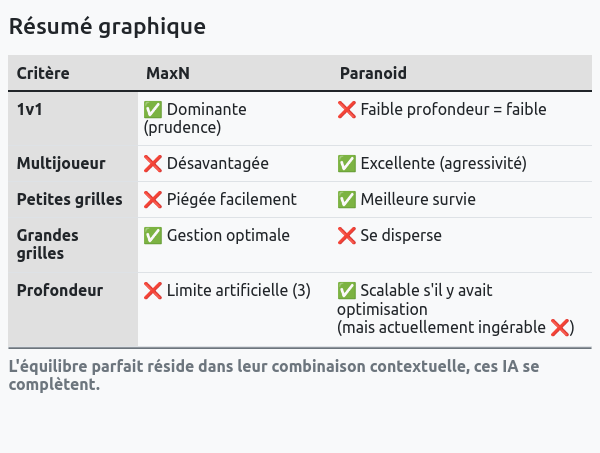
\includegraphics[width=0.5\linewidth]{TableauResumeIA}
		\end{figure}
		
\newpage

\section{Amélioration effectués}

\subsection{Jeu jouable par utilisateur}
Le modèle-vue-contrôleur possède une classe TerminalControlleur, cette classe permet de récupérer la direction souhaité du joueur en écrivant celle-ci grâce au terminal de jeu.

\subsection{MVC}
L'utilisation de ce concept dans ce projet me permet de pouvoir effectuer des modifications isolées assez facilement, plus simple à debugger car modèle indépendant de la vue et pour finir le projet possède une bonne extensibilité afin d'ajouter de nouvelles IA ou vues sans se prendre la tête.

\subsection{Optimisation de MaxN}
Cette optimisation baisse un peu l'efficacité de l'IA lorsque la profondeur augmente mais lui donne l'avantage d’être rapide et tout en restant efficace pour jouer en temps réel.

\subsection{Modèle Observeur-Observable}
Le premier avantage est le découplage des composants. Je peux donc changer l'Observeur ou l'Observable sans impacter l'autre.
La réactivité et la mise à jour est dynamique. L'extensibilité est facilitée. Ça permet aussi la cohérence des données et économise le CPU en évitant les vérifications manuelles.

\subsection{Outils d’expérimentations}
Afin de bien mener mes expérimentations j'ai crée un nouveau package composé de trois classes. Elles testent toutes différentes catégories de statistiques qui sont les suivantes: taux de victoire, durée moyenne d'une partie et temps de calcul moyen d'un IA pour jouer son coup.
Ces classes sont efficaces, ont un affichage complet et sont faciles à paramétrer.

\subsection{Super Build.xml}
Je possède actuellement 1 build.xml par package et j'en ai créer un autre général pour tout gérer plus facilement à partir de celui-ci.
Voici les commandes disponibles:
\begin{itemize}
\item ant javadoc (compilation, javadoc)
\item ant jar (compilation, copy.jar, .jar executable)
\item ant run (jar + execute le jeu)
\item ant runWinrate | runTemps | runSurvie (execute un outil d'experimentation)
\end{itemize}

\subsection{Javadoc}
Génération d'une documentation technique claire et à jour directement à partir du code source.

\section{Conclusion finale}
Ce projet m'a permit d'explorer les dynamiques complexes du jeu de Tron multi-joueur en étudiant l'influence des coalitions, de la profondeur de recherche et de la taille de la grille sur les performances des IA. À travers l'implémentation des algorithmes MAXN et Paranoid, j'ai pu comparer deux approches stratégiques distinctes : l'une optimisant les gains individuels au sein d'une équipe, l'autre adoptant un comportement agressif en considérant tous les autres joueurs comme des adversaires.

Mes expérimentions ont révélé que:
La profondeur de recherche joue un rôle crucial dans l'efficacité des IA, avec des performances qui s'améliorent significativement à mesure que la profondeur augmente (théoriquement pour MaxN), bien que cela rend ingérable les temps de calculs de Paranoid.
La taille des équipes influence la balance du jeu, MaxN est dominante en 1v1 et Paranoid est meilleure en coalition.
La taille de la grille détermine l'avantage stratégique, les petites grilles favorisent les réactions rapides et les blocages ce qui permet à Paranoid de rivaliser et expansion de la grille permet à MaxN d'écraser stratégiquement Paranoid.

Les résultats obtenus ouvrent la voie à des améliorations potentielles, comme l'optimisation de Paranoid afin d'éviter l'explosion de temps de calcul quand la profondeur augmente. On pourrait aussi imaginer un mode de jeu IA vs Joueur. A propos de l'interface graphique pourrait permettre de contrôler le joueur, elle pourrait aussi mieux afficher quel mur a été posé par quel joueur, en donnant une couleur pour chaque joueurs pour son Tron et ses Murs et pour finir on pourrait imaginer une Vue et un Contrôleur qui fonctionneraient en réseau.

En conclusion, ce projet m'a permis d'appliquer des concepts de programmation orientée objet, ainsi que des techniques de conception logicielle telles que l'architecture MVC
et les design patterns. Cela a été une excellente occasion d'améliorer mes compétences en
programmation et de renforcer ma compréhension des principes du génie logiciel et de l'IA. Le
fait d'avoir travaillé seul m'a aussi permis de toucher à tout et donc d'appendre d'avantage sur tous les domaines en plus d'orienter le projet dans la direction que je souhaitais sans contraintes. Bien qu'en contre partie mon travail personnel a été davantage important.
\end{document}